%!TEX root = ../report.tex

\begin{document}
    \chapter{Hand crafted feature extraction}
This chapter discusses the experiments conducted based on methods present in chapter 5 section 5.1. 
 

\subsection{Objective}
Objective of this experiment is to extract a fixed set of features from each of the signal acceleration, velocity and position. From this fixed set relevant features will be selected and classified using state of art machine learning algorithms.

\section{Experiment details}
As the data is imbalanced therefore to perform data balancing following set of data division is performed. Following table describes data balancing experiments performed.

\begin{table}[h]
\begin{tabular}{|l|l|l|l|}
	\hline
	Data division & Details                                                                      & Positive samples & Negative samples \\ \hline
	D1            & \begin{tabular}[c]{@{}l@{}}The data is divided in 1:1 \\ ratio.\end{tabular} & 103              & 103              \\ \hline
	D2            & The data is slightly biased 2:1                                              & 206              & 103              \\ \hline
	
\end{tabular}
	\caption{Data division for balancing}
\end{table}
    
 The number of features selected varies as follows:
 \begin{itemize}
 \item First feature set is defined as  feature selection based on relevance let us call it as F1. 
 \item To analyze the effect of the prior domain knowledge features, set of two is selected that is penetration and maximum velocity. Let us call this F2.
 \end{itemize} 
 
 \section{Results} 
 
 The relevance of the features can be visualized as follows:
   \begin{figure}[h]
   	\centering
   	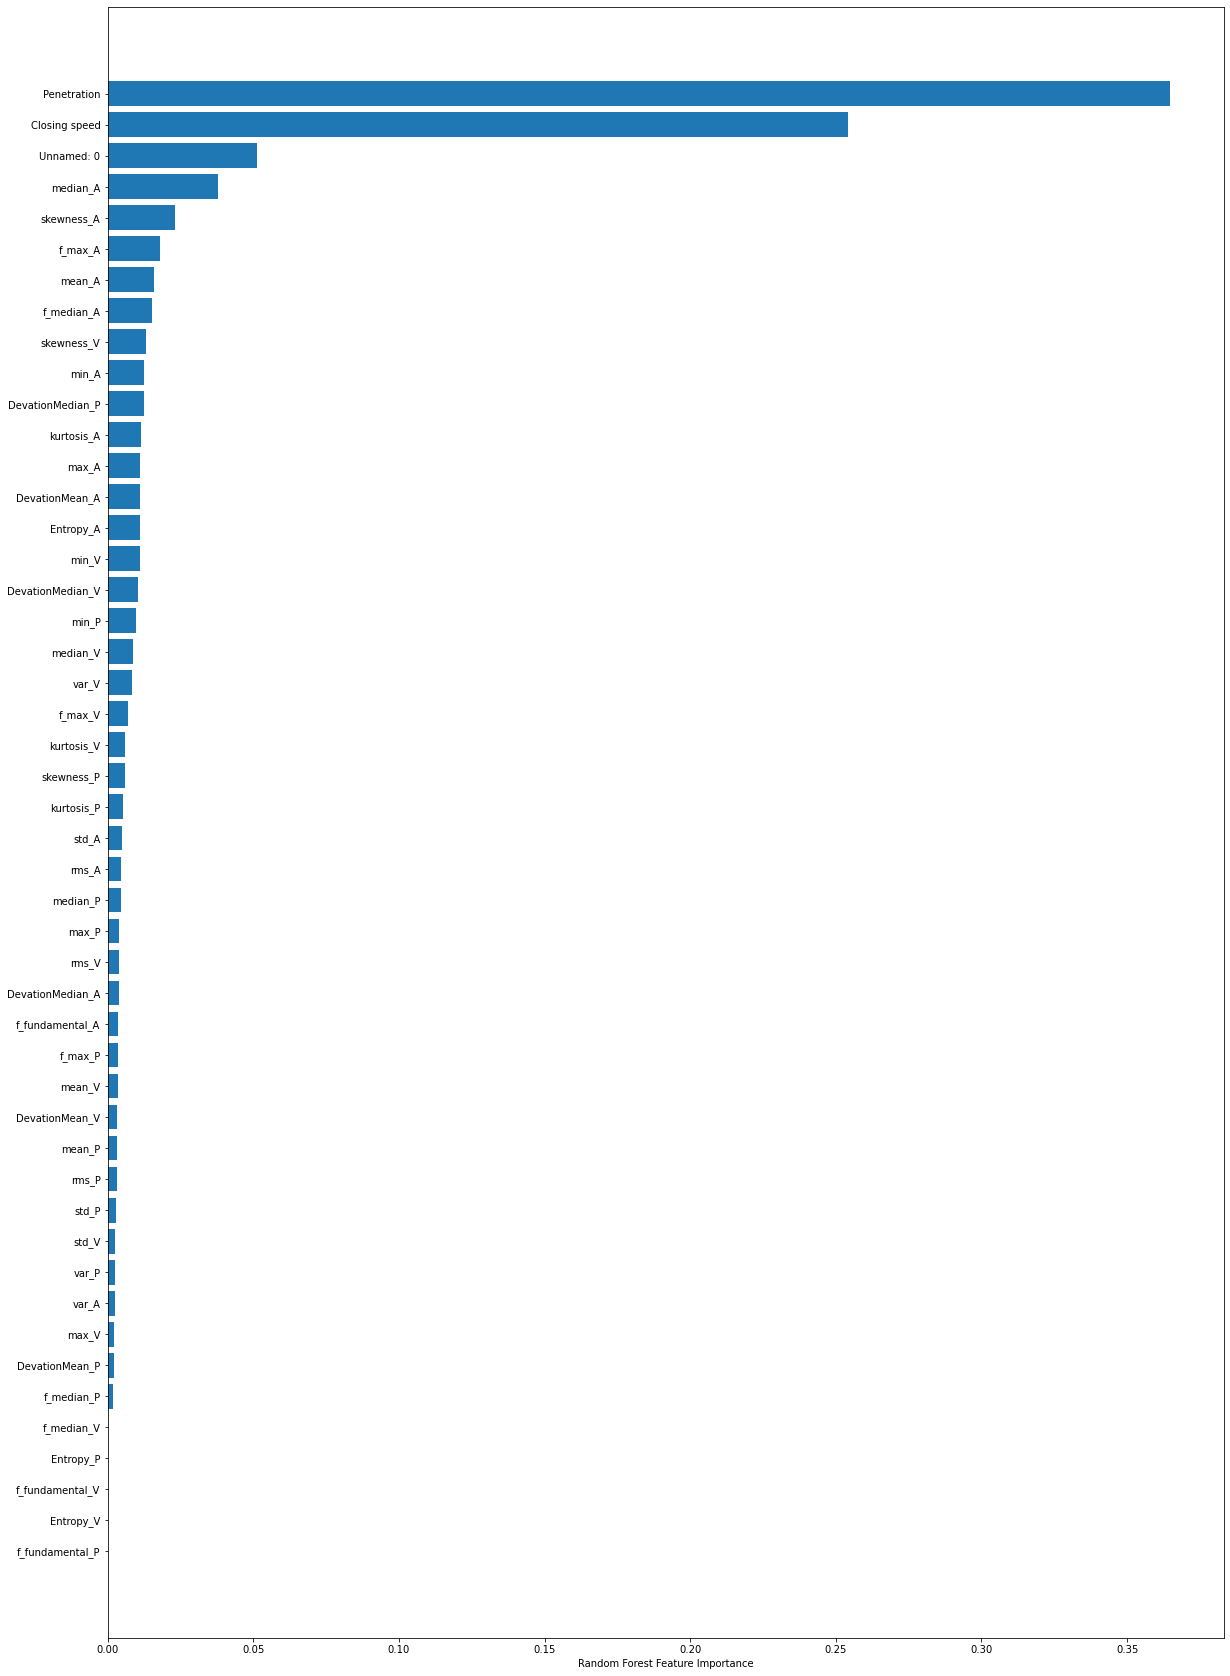
\includegraphics[width=0.62\linewidth]{images/relvance.png}
   	\caption{Relevance of features}
   	\label{n5}
   \end{figure}
Results related to data division D1 and D2 category are presented as in figure \ref{r1} and \ref{r2}:  
      \begin{figure}[b]
      	\centering
      	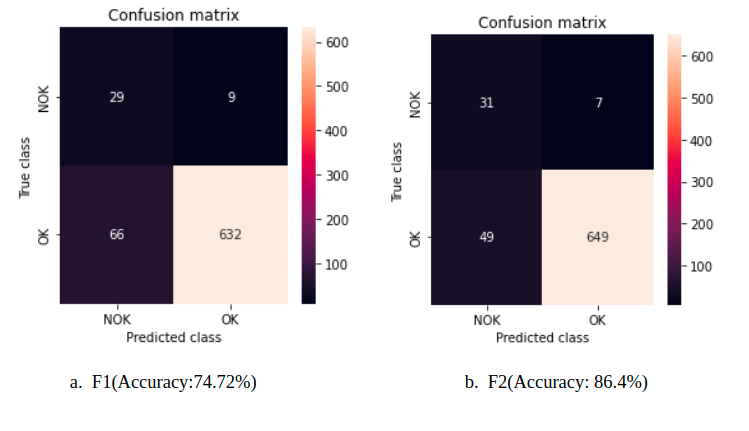
\includegraphics[width=1\linewidth]{images/r1.png}
      	\caption{Results for D1 category}
      	\label{r1}
      
      \end{figure}
         \begin{figure}[b]
         	\centering
         	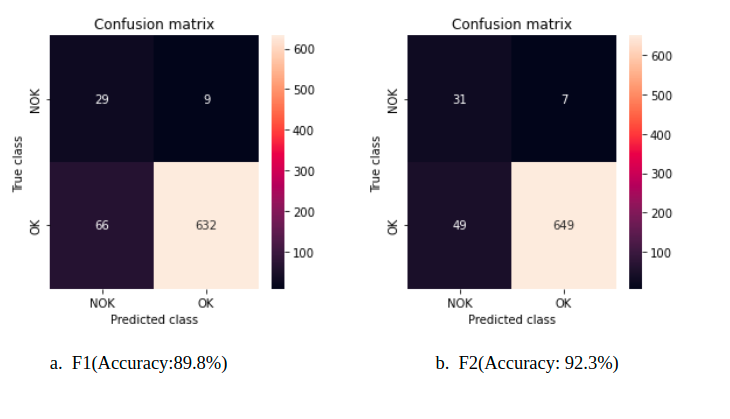
\includegraphics[width=1\linewidth]{images/r2.png}
         	\caption{Results for D2 category}
         	\label{r2}
         \end{figure}
  Parameters related to the Testing  data:
  \begin{itemize}
  	\item Positive samples: 698
  	
  \item	Negative Samples:38
  	
  \end{itemize}
 
  \section{Discussions}      
  
  As observed the algorithm performs better for  when the prior knowledge is used that is the F2 category. Both the categories show no significant difference in number of negative samples obtained by the algorithms. This shows that the prior domain knowledge has high influence on negative sample detection. 

  \chapter{Autoencoder for anomaly detection}
  This chapter discusses the experiments conducted based on methods present in chapter 5 section 5.2. 
  \section{Objective}
  Aim of this experiment is to use reconstruction error as base to classify the data into normal and abnormal. This experiment does not consider the labels assigned that is, its a unsupervised learning algorithm. The details of architecture have been discussed in section 5.2. 
  This experiment is conducted on each type of signal to analyze which signal has better features that encode the anomaly.
  
  \section{Results}  
  
  \subsection{Trained with positive data:T1}
   Parameters related to the  data distribution:
  \begin{table}[h]
  	\begin{tabular}{|l|l|l|}
  		\hline
  		Data      & Positive samples & Negative samples \\ \hline
  		Train set & 2311             & 0                \\ \hline
  		Test set  & 1848             & 112              \\ \hline
  	\end{tabular}
  	\caption{Parameters for T1}
  \end{table}
   	    \begin{figure}[h]
   	    	\centering
   	    	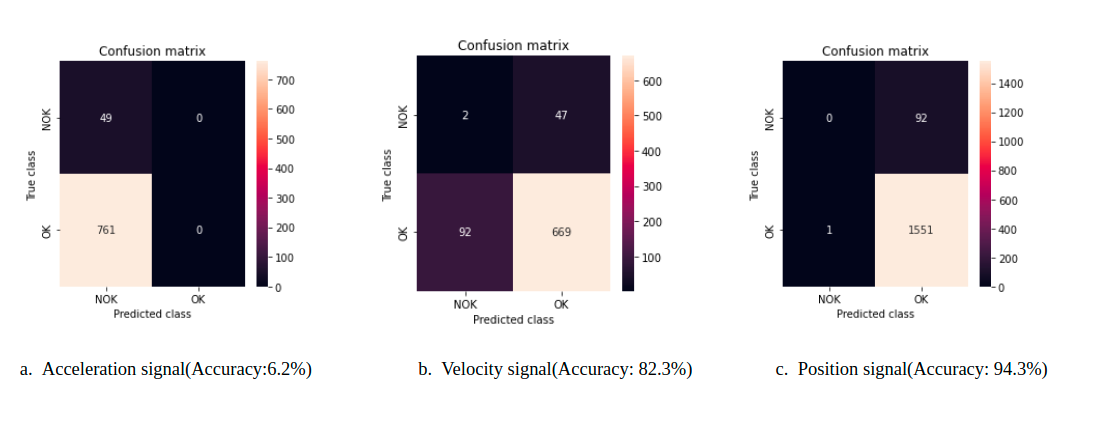
\includegraphics[width=1\linewidth]{images/r3.png}
   	    	\caption{Results for T1}
   	    	\label{r3}
   	    \end{figure}
   	
     \subsection{Trained with combination of positive  and negative data: T2}
     
       \begin{table}[h]
       	\begin{tabular}{|l|l|l|}
       		\hline
       		Data      & Positive samples & Negative samples \\ \hline
       		Train set & 1550             & 761              \\ \hline
       		Test set  & 1848             & 34              \\ \hline
       	\end{tabular}
       	\caption{Parameters for T2}
       \end{table}
        \begin{figure}[h]
        	\centering
        	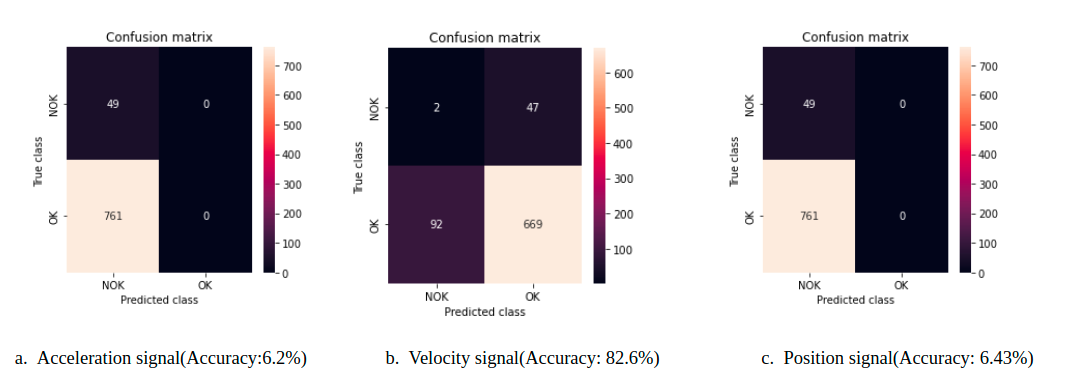
\includegraphics[width=1\linewidth]{images/r4.png}
        	\caption{Results for T2}
        	\label{llll}
        \end{figure}
        
       \begin{figure}[t]
       	\centering
       	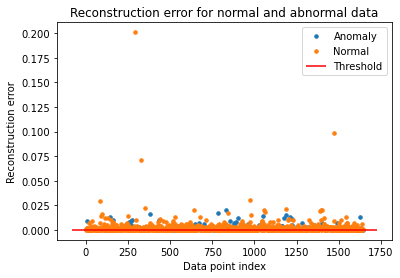
\includegraphics[width=0.8\linewidth]{images/download.png}
       	\caption{Reconstruction error distribution}
       	\label{lll}
       	
       \end{figure}
   \section{Discussions} 
   As it can be visualized from the \ref{r3} and \ref{lll} even though the accuracy of the experiments for velocity is high it fails to detect abnormal data. The reason behind this could due to the reconstruction error of the anomalies is very close to normal ones. This can be visualized in figure \ref{lll}. Optimal threshold cannot be decided due to this issue as if we increase the threshold most of the normal data will be classified as abnormal. Therefore the threshold is kept very low and it can be observed in the confusion plots that most of abnormal data is been classified as normal.
   
   
   \chapter{Transfer learning}
   
   \section{Signal as input}
   
   \subsection{Objective}
   
   Objective of this experiment is to use convolution neural network pre-trained with UCR datasets as base model for feature extraction from comfort door acceleration data. 
   The results 
       
\end{document}
